\section{Experiments and Results}
\label{sec:experiments}


\begin{table*}[t]
% \small
    \centering
\resizebox{1\textwidth}{!}{%
\begin{tabular}{lllllllll}
\toprule
Models &       LAMA & Group-Score &    Succ-Pat &  Succ-Objs &  Know-Const &   Unk-Const &  Const-Objs & Consistency \\

\midrule
majority-baseline &  24.2+-20.7 &  24.2+-20.7 &  100.0+-0.0 &  24.9+-20.7 &  100.0+-0.0 &  100.0+-0.0 &  100.0+-0.0 &  100.0+-0.0 \\ \midrule
bert-base         &  44.1+-25.6 &  25.0+-25.5 &  100.0+-0.0 &  60.6+-23.5 &  61.4+-23.2 &  45.2+-20.6 &  32.5+-28.5 &  57.3+-22.3 \\
bert-large        &  45.6+-27.0 &  27.5+-27.6 &   99.7+-1.8 &  63.0+-25.2 &  62.4+-22.4 &  46.4+-18.5 &  34.2+-30.0 &  59.1+-21.5 \\
bert-large-wwm    &  45.4+-26.4 &  27.2+-27.6 &  100.0+-0.0 &  61.6+-23.2 &  62.6+-23.6 &  46.5+-18.7 &  33.8+-29.8 &  58.6+-22.7 \\ \midrule
roberta-base      &  36.7+-24.6 &  16.0+-19.8 &  100.0+-0.0 &  54.2+-24.5 &  53.3+-20.2 &  41.2+-15.3 &  21.7+-23.1 &  50.1+-18.4 \\
roberta-large     &  40.8+-26.1 &  21.3+-23.7 &  100.0+-0.0 &  58.5+-24.1 &  58.2+-21.1 &  44.4+-16.0 &  27.4+-25.6 &  54.8+-19.6 \\ \midrule
albert-base       &  29.9+-24.2 &  17.0+-22.2 &   99.7+-1.8 &  45.3+-25.7 &  56.1+-21.5 &  43.1+-18.0 &  25.1+-25.4 &  51.2+-19.8 \\
albert-xxlarge    &  39.5+-26.1 &  21.9+-25.7 &   99.7+-1.8 &  56.3+-25.8 &  56.7+-22.7 &  38.8+-14.7 &  26.8+-26.8 &  51.5+-21.1 \\
\bottomrule
\end{tabular}


}
    \caption{Consistency and knowledge results for the different models.}
    \label{tab:consistency_main}
\end{table*}

\subsection{Consistency}

The results for the different models are summarized in Table \ref{tab:consistency_main}.
% First, we report the average consistency results for all graphs, as describe in Section \ref{sec:eval}.
The last column (``Consistency'') shows the average results across all relations \yg{consider oredering the table columns in the order of their discussion}\am{I actually like it in the end, its easier to find in a glance}

The BERT-based models achieve higher scores over all the models\am{over the others, or the rest}. Moreover, there is a consistent improvement from the base to large\am{emph or quote 'base' and 'large'} versions of each model, although it is not always significantly \am{is there a significance test?} higher (e.g. 57.3\% to 59.1\% in BERT, and 50.1\% to 54.8\% in RoBERTa).
However, in contrast to many previous works that observed quantitative and qualitative improvements of RoBERTa-based models over BERT, in terms of consistency\am{comma} BERT is better than RoBERTa and ALBERT.\am{I would rephrase and say "BERT is more consistent than ...."}
Still, the overall results are remarkably low (59.1\% for the best model, \yg{meaning that out of XXX, YYY are ZZZ}), especially given the permissive evaluation that only looks at the candidate set.
We note that the results are highly variant between models and relations. For instance, the best performing model on the `capital of' relation achieves 94\%, whereas the best performing model on `owned by' is 44\%\am{is what? "achieves"?}. 
On the other hand, the models' performance on the `original language of film or TV show' relation, varies between 52\% and 90\% accuracy.
We report the full consistency results for each relation in the Appendix.

\begin{table}[t]
% \small
    \centering
\resizebox{1\columnwidth}{!}{%
\begin{tabular}{lrrr}
\toprule
Model&        Acc & Consistency & Consistent-Acc \\

\midrule
majority               &  23.1+-21.0 &  100.0+-0.0 &  23.1+-21.0 \\
\midrule
RoBERTa-med-small-1M &   11.2+-9.4 &  37.1+-11.0 &    2.8+-4.0 \\
\midrule
RoBERTa-base-10M     &  17.3+-15.8 &  29.8+-12.7 &    3.2+-5.1 \\
RoBERTa-base-100M    &  22.1+-17.1 &  31.5+-13.0 &    3.7+-5.3 \\
RoBERTa-base-1B      &  \textbf{38.0}+-23.4 &  \textbf{50.6}+-19.8 &  \textbf{18.0}+-16.0 \\
\bottomrule
\end{tabular}
}
    \caption{Knowledge and consistency results for the different RoBERTas, trained on increasing amounts of data. Best model for each metric is highlighted in bold.}
    \label{tab:robertas}
\end{table}

% \enote{hs}{below: i would prefer ``(training) corpus size''
%   over ``number of tokens'' if that's what you mean}

\paragraph{Effect of Pretraining Corpus Size}
Next, we study the question of whether the number of tokens used during the pretraining contributes to consistency.
We use the pretrained RoBERTas model provided by \citet{robertas} and repeat the experiments on four additional models.
These models are RoBERTa-based models, that were trained on a sample of Wikipedia and the book corpus, with varying training size, and parameters. In practice, we use one of the three published models for each configuration and report the average accuracy over the relations for each model in Table \ref{tab:robertas}.
Overall, the consistency and the knowledge scores (LAMA and Group-Score) improve when trained on more data. \nk{Maybe I missed it, did we say what the Group-Score is before?}\am{seems like not} However, there is an interesting outlier to this trend.
First, the model that was trained on one million tokens is more consistent than the models trained on ten and one-hundred million tokens. A potentially crucial difference is that this model is also smaller in terms of the number of parameters than the rest, in order to avoid overfitting. Still, it is nonetheless interesting that a model that is trained on significantly fewer\am{I would use "less"} data can achieve better consistency. On the other hand, the knowledge scores are lower, arguably due to less factual knowledge this model was exposed to during training.\am{due to the model being exposed to less factual knowledge during pretraining}

% Finally, the original RoBERTa that was trained on ten billion parameters, achieves the same consistency performance as the one trained on one billion tokens, suggesting a limit to the benefit of training examples in pretraining. \nk{not sure about this as the table is not there yet, but shouldn't it be: Finally, the original RoBERTa that was trained on ten billion tokens, achieves the same consistency performance as the one trained on one billion tokens, suggesting on a limit to the benefit of large training corpora. }



% \begin{table*}[t]
% \small
    \centering
\resizebox{1\textwidth}{!}{%
\begin{tabular}{lrrrrrrr}
\toprule
{} &  bert-base &  bert-large &  bert-large-wwm &  roberta-base &  roberta-large &  albert-base &  albert-xxlarge \\
\midrule
syn   &             0.50 &              0.53 &                                 0.53 &          0.44 &           0.48 &            0.44 &               0.45 \\
lex   &             0.56 &              0.59 &                                 0.58 &          0.51 &           0.54 &            0.52 &               0.49 \\
both  &             0.72 &              0.72 &                                 0.72 &          0.67 &           0.68 &            0.70 &               0.63 \\ \midrule
total &             0.52 &              0.54 &                                 0.54 &          0.45 &           0.50 &            0.46 &               0.46 \\
\bottomrule
\end{tabular}


}
    \caption{Consistent results aggregated on the different relations, by the different splits.}
    \label{tab:entailment-splits}
\end{table*}

% \begin{table*}[t]
% \small
    \centering
\resizebox{1\textwidth}{!}{%
\begin{tabular}{llrrrrrrr}
\toprule
     type & index &  bert-base-cased &  bert-large-cased &  bert-large-cased-wwm &  roberta-base &  roberta-large &  albert-base &  albert-xxlarge \\
\midrule
\multirow{3}{*}{consistency} & 1-1 &             0.76 &              0.82 &                                 0.84 &          0.58 &           0.73 &            0.66 &               0.80 \\
     & N-1 &             0.55 &              0.56 &                                 0.57 &          0.48 &           0.51 &            0.46 &               0.48 \\
     & N-M &             0.43 &              0.47 &                                 0.46 &          0.39 &           0.44 &            0.44 &               0.40 \\
\cline{1-9}
\multirow{3}{*}{syntactic} & 1-1 &             0.75 &              0.81 &                                 0.83 &          0.57 &           0.72 &            0.66 &               0.79 \\
     & N-1 &             0.53 &              0.55 &                                 0.56 &          0.46 &           0.49 &            0.44 &               0.47 \\
     & N-M &             0.41 &              0.45 &                                 0.44 &          0.38 &           0.43 &            0.42 &               0.40 \\
\cline{1-9}
\multirow{3}{*}{lexical} & 1-1 &             0.85 &              0.88 &                                 0.89 &          0.67 &           0.80 &            0.75 &               0.86 \\
     & N-1 &             0.59 &              0.60 &                                 0.62 &          0.55 &           0.57 &            0.51 &               0.51 \\
     & N-M &             0.45 &              0.53 &                                 0.48 &          0.40 &           0.44 &            0.52 &               0.39 \\
\cline{1-9}
\multirow{3}{*}{both} & 1-1 &             0.59 &              0.76 &                                 0.83 &          0.16 &           0.49 &            0.46 &               0.73 \\
     & N-1 &             0.75 &              0.76 &                                 0.74 &          0.69 &           0.72 &            0.72 &               0.69 \\
     & N-M &             0.68 &              0.66 &                                 0.68 &          0.64 &           0.64 &            0.68 &               0.54 \\
\bottomrule
\end{tabular}

}
    \caption{Consistent results aggregated on the different relations, by the different splits.}
    \label{tab:entailment-splits}
\end{table*}


% \begin{figure*}[t!]
% \centering

% 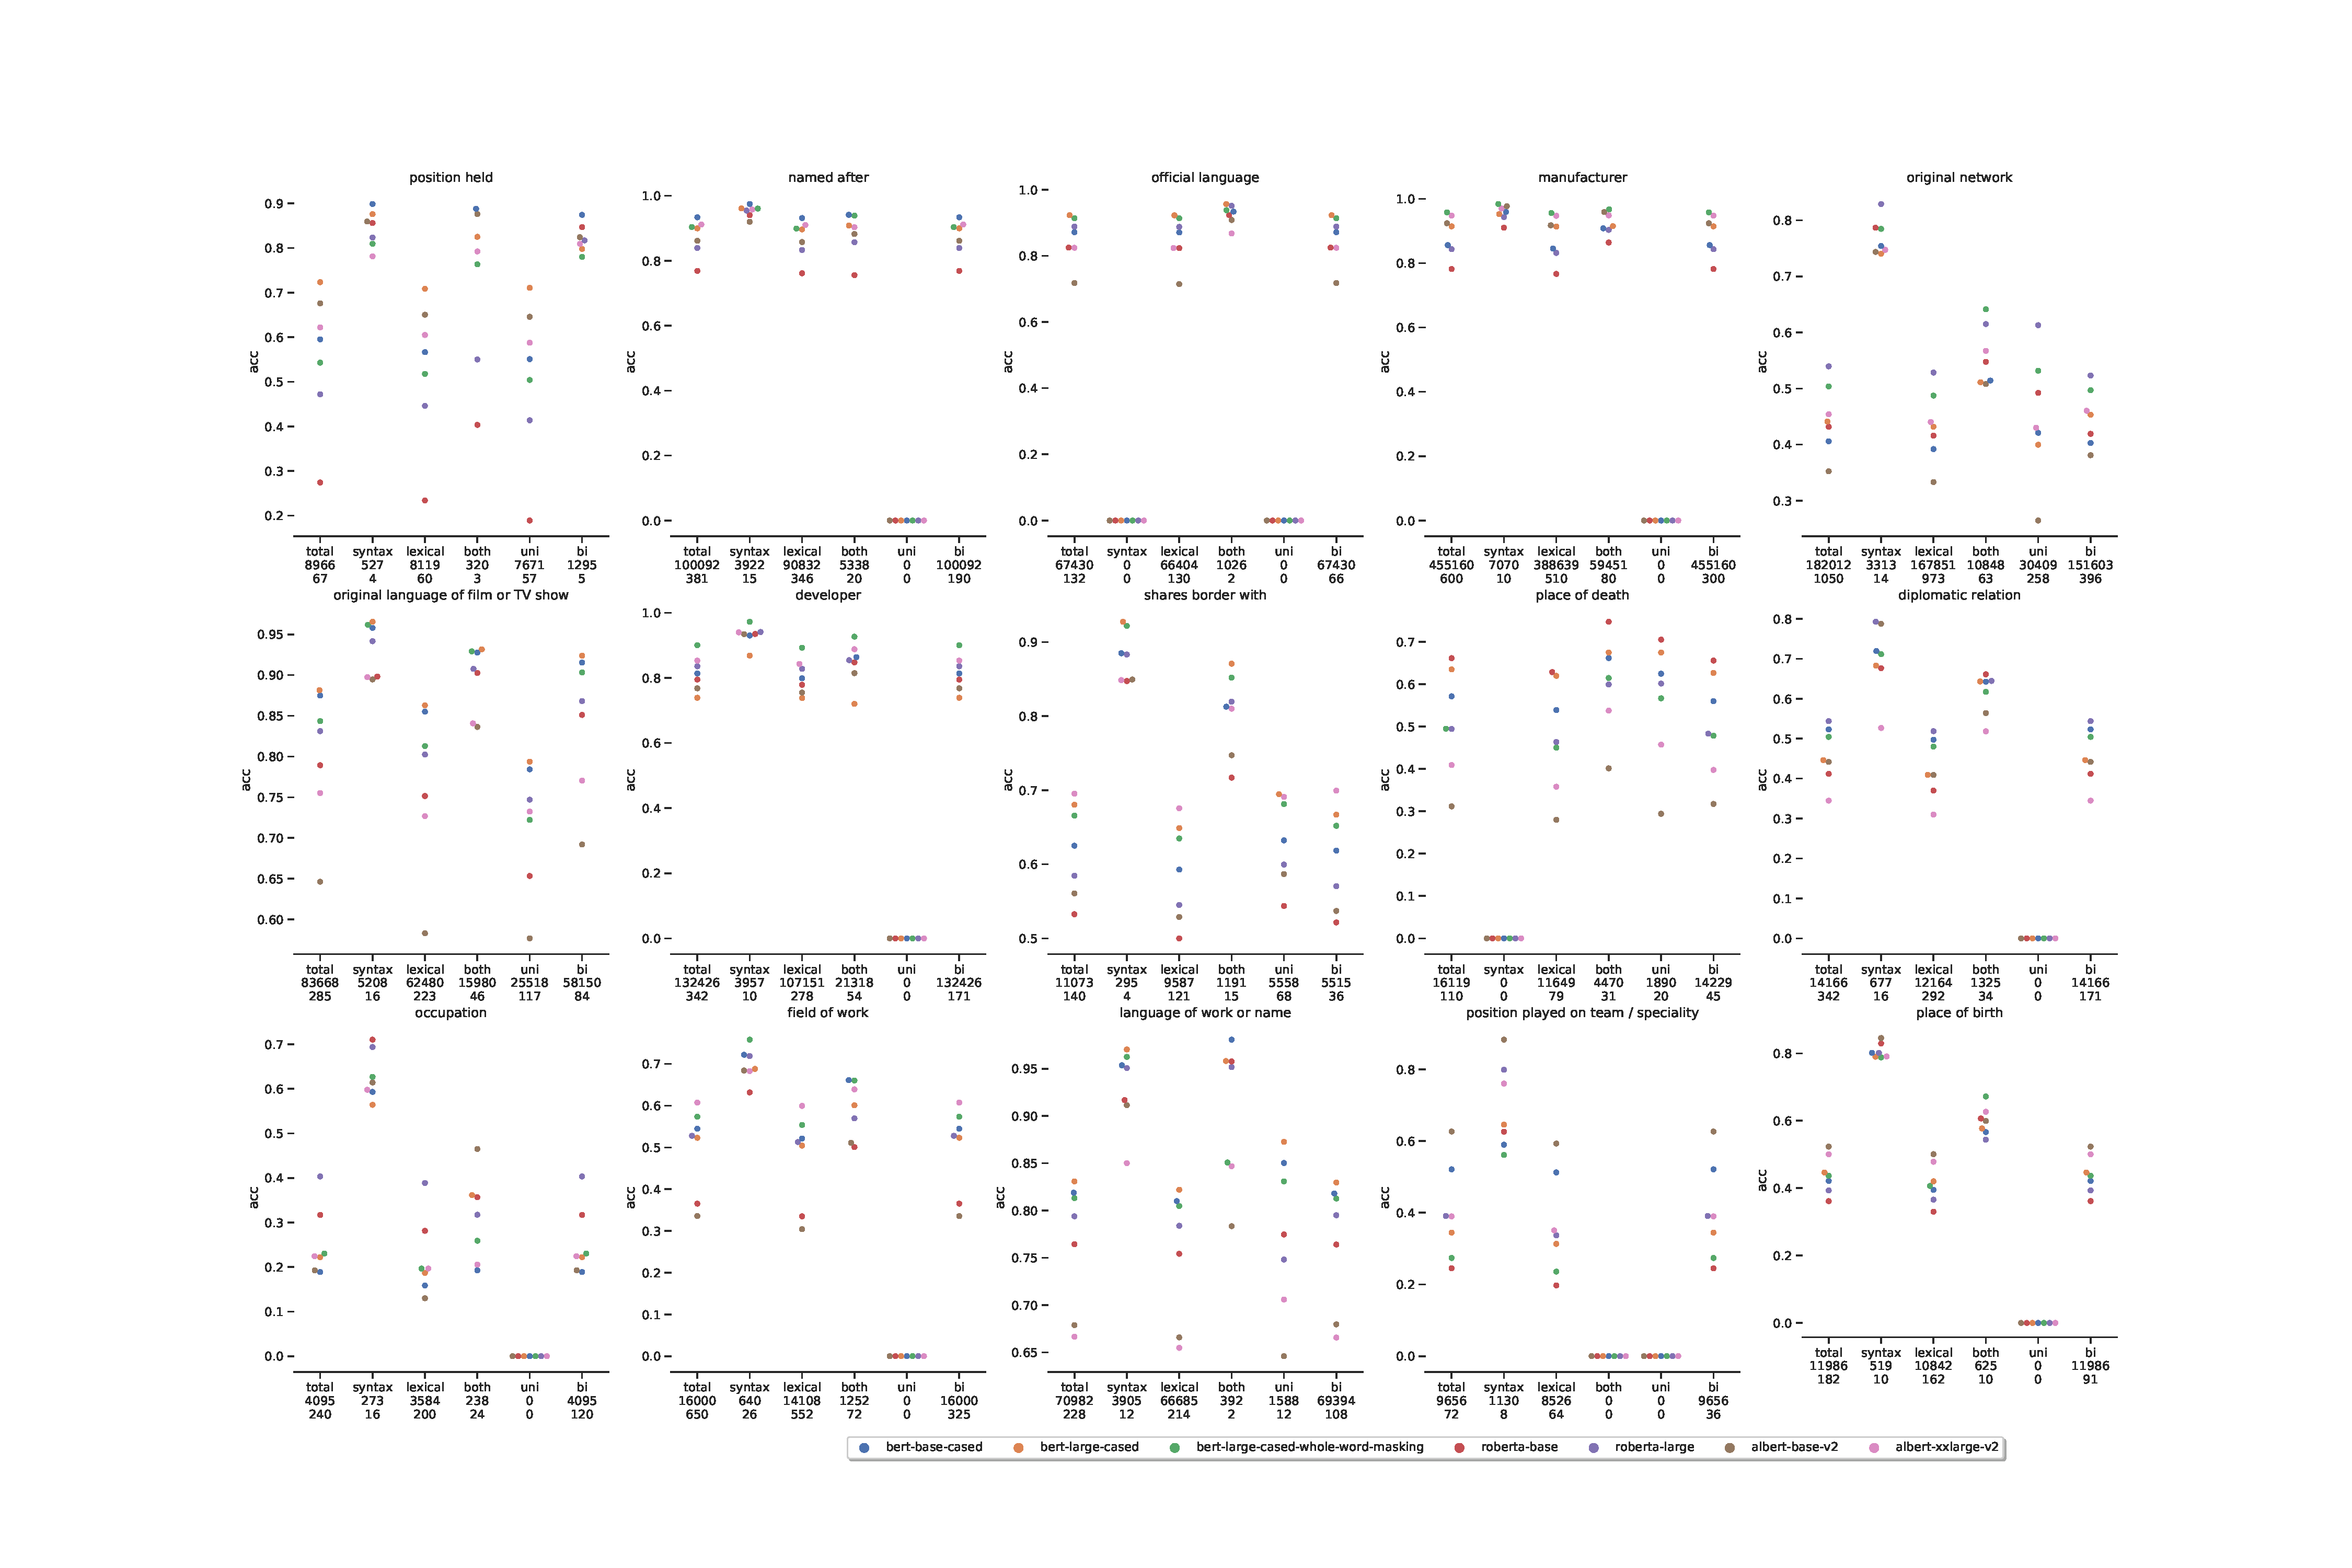
\includegraphics[width=1.\textwidth]{figures/results}

% \caption{Results summary, by relation, by split.}
% \label{fig:resuls}
% % \vspace{-6mm}
% \end{figure*}

% \begin{table*}[t]
% \small
    \centering
\resizebox{1\textwidth}{!}{%
\begin{tabular}{lrrrrrrrr}
\toprule
                              pattern &  know &  unk &  top@1 &  group-score &  const-subjs &  succ-patt &  succ-subjs &  consistency \\
\midrule
                             religion &                      0.35 &                        0.22 &      0.12 &            0.09 &                 0.09 &                  1.0 &                 0.88 &         0.34 \\
                       place of death &                      0.43 &                        0.32 &      0.42 &            0.04 &                 0.05 &                  1.0 &                 0.54 &         0.38 \\
                              capital &                      0.91 &                        0.40 &      0.70 &            0.57 &                 0.61 &                  1.0 &                 0.75 &         0.78 \\
                           instrument &                      0.48 &                        0.62 &      0.50 &            0.03 &                 0.05 &                  1.0 &                 0.85 &         0.50 \\
                             employer &                      0.38 &                        0.38 &      0.10 &            0.03 &                 0.11 &                  1.0 &                 0.27 &         0.38 \\
                headquarters location &                      0.65 &                        0.35 &      0.36 &            0.21 &                 0.25 &                  1.0 &                 0.53 &         0.51 \\
                        position held &                      0.49 &                        0.46 &      0.29 &            0.08 &                 0.11 &                  1.0 &                 0.65 &         0.48 \\
                            continent &                      0.92 &                        0.74 &      0.90 &            0.83 &                 0.85 &                  1.0 &                 0.97 &         0.91 \\
                            member of &                      0.92 &                        0.27 &      0.84 &            0.72 &                 0.74 &                  1.0 &                 0.89 &         0.85 \\
                              country &                      0.89 &                        0.74 &      0.60 &            0.54 &                 0.77 &                  1.0 &                 0.65 &         0.84 \\
                          subclass of &                      0.83 &                        0.53 &      0.61 &            0.56 &                 0.63 &                  1.0 &                 0.78 &         0.76 \\
                          instance of &                      0.51 &                        0.19 &      0.53 &            0.05 &                 0.05 &                  1.0 &                 0.86 &         0.47 \\
                              part of &                      0.62 &                        0.53 &      0.47 &            0.31 &                 0.57 &                  1.0 &                 0.51 &         0.57 \\
                             owned by &                      0.55 &                        0.23 &      0.51 &            0.21 &                 0.22 &                  1.0 &                 0.65 &         0.44 \\
                         record label &                      0.26 &                        0.28 &      0.06 &            0.00 &                 0.00 &                  1.0 &                 0.79 &         0.26 \\
                        field of work &                      0.28 &                        0.21 &      0.15 &            0.01 &                 0.01 &                  1.0 &                 0.39 &         0.23 \\
                        work location &                      0.74 &                        0.68 &      0.42 &            0.28 &                 0.42 &                  1.0 &                 0.59 &         0.72 \\
             language of work or name &                      0.70 &                        0.60 &      0.72 &            0.21 &                 0.23 &                  1.0 &                 0.85 &         0.69 \\
          twinned administrative body &                      0.57 &                        0.70 &      0.04 &            0.02 &                 0.37 &                  1.0 &                 0.07 &         0.69 \\
                         manufacturer &                      0.88 &                        0.33 &      0.90 &            0.62 &                 0.62 &                  1.0 &                 0.96 &         0.86 \\
                location of formation &                      0.59 &                        0.50 &      0.11 &            0.03 &                 0.13 &                  1.0 &                 0.18 &         0.52 \\
                                genre &                      0.52 &                        0.41 &      0.61 &            0.03 &                 0.03 &                  1.0 &                 0.79 &         0.49 \\
                    official language &                      0.87 &                        0.70 &      0.64 &            0.49 &                 0.64 &                  1.0 &                 0.81 &         0.84 \\
 position played on team / speciality &                      0.30 &                        0.32 &      0.06 &            0.00 &                 0.00 &                  1.0 &                 0.45 &         0.31 \\
                            developer &                      0.63 &                        0.28 &      0.71 &            0.22 &                 0.22 &                  1.0 &                 0.91 &         0.60 \\
                             location &                      0.56 &                        0.34 &      0.49 &            0.01 &                 0.01 &                  1.0 &                 0.70 &         0.49 \\
                          named after &                      0.78 &                        0.47 &      0.60 &            0.38 &                 0.41 &                  1.0 &                 0.80 &         0.71 \\
                    country of origin &                      0.67 &                        0.54 &      0.40 &            0.20 &                 0.25 &                  1.0 &                 0.63 &         0.62 \\
                     original network &                      0.29 &                        0.25 &      0.33 &            0.00 &                 0.00 &                  1.0 &                 0.82 &         0.28 \\
                       place of birth &                      0.46 &                        0.38 &      0.26 &            0.00 &                 0.01 &                  1.0 &                 0.32 &         0.41 \\
              applies to jurisdiction &                      0.94 &                        0.69 &      0.76 &            0.74 &                 0.82 &                  1.0 &                 0.83 &         0.90 \\
                           occupation &                      0.34 &                        0.35 &      0.01 &            0.00 &                 0.00 &                  1.0 &                 0.14 &         0.35 \\
                           capital of &                      0.95 &                        0.51 &      0.89 &            0.80 &                 0.82 &                  1.0 &                 0.92 &         0.92 \\
 original language of film or TV show &                      0.89 &                        0.90 &      0.58 &            0.50 &                 0.79 &                  1.0 &                 0.64 &         0.90 \\
               country of citizenship &                      0.74 &                        0.65 &      0.36 &            0.27 &                 0.32 &                  1.0 &                 0.68 &         0.71 \\
                   shares border with &                      0.54 &                        0.54 &      0.26 &            0.06 &                 0.14 &                  1.0 &                 0.54 &         0.54 \\
\bottomrule
\end{tabular}
}
    \caption{Additional results for the BERT-large model. }
    \label{tab:bert-results}
\end{table*}


\subsection{Consistency and Knowledge}

\yg{wdym by ``to asses the knowledge and ability of the different patterns to extract knowledge''? in particular, what is the first `knowledge'?}
To better understand the results, and assess the knowledge and ability of the different patterns to extract the correct knowledge of \resource{}, we report additional metrics that help to\am{remove "to"? unsure} understand the results. \sr{need a better motivation. e.g. ``In this section, we provide a finer-grained analysis, measuring consistency scores in various settings". But honestly this looks a bit like a checklist of different, unrelated experiments, and may be better pushed into an appendix.}

First, we report the percentage of triples that were predicted correctly by at least one of the patterns (Succ-Objs), and the percentage of patterns that successfully predicted the right object at least once (Succ-Patt). Succ-Objs quantifies the degree to which the knowledge is stored by the models, and Succ-Patt quantified the quality of the patterns to extract the knowledge.
Across models, all patterns successfully extracted the right
answer at least once, except for three models (bert-large and the two versions of albert) where one pattern in the `diplomatic relation'  did not succeed to classify any tuple.
On the other hand, some tuples are not predicted correctly by any of the patterns, as is shown in the Succ-Objs measure. Since most relations contain at least @@ patterns, we take it as evidence that this knowledge is not stored in the model. 
% \nk{This seems to suggest that it is the fault of the pattern that knowledge is not extracted from the model but an unsuccessful prediction across all models of the same tuple rather says that this knowledge is not stored} 
The average number of extractable tuples \am{extractable tuples?} is between 45.3\% to 63.0\%, depending on the model. Notably, the BERT based models are consistently better than the rest in extracting the knowledge. 

Next, we report LAMA results, that is\am{comma} the acc@1 accuracy\am{acc@1 accuracy is weird} of a model in predicting the object, using the original patterns from \citet{lama}. This metric inspects whether the first object within the candidate set of each relation is the correct answer. The reported numbers for this metric differ from \citet{lama} \am{reporting X\%} as we use a candidate set, as well as take only the KB triple where the objects are a single token in all models we inspect. The results range between 29.9 with albert-base to 45.6\am{should be \%?} with bert-large, being the best model in that aspect.
Additionally, we report another metric, which we call \textsc{Group-Score}, where a point is given only when all patterns predict the object correctly. This metric is much stricter than \textit{acc@1}, however, it provides a more robust metric, and better quantifies the degree to which the knowledge is encoded into the model. Overall, it combines both the requirement of a model to be consistent and correct. The results are much lower than the LAMA metric, as expected, but follow the same trend: albert-base perform worse, 17.0\% and bert-large performs best with 27.5\% accuracy.

\yg{give this part a paragraph title?}
Next, we measure the consistency results for the tuples
subset where at least one of the patterns for a specific
relation predicted the correct answer, as well as for the
subset where no pattern predicted the right answer correctly \am{correct answer, like previous line}
-- we refer to these metrics as \textsc{Know-Const} and \textsc{Unk-Const}, respectively.
A higher score on the first metric would suggest that storing the correct answer is related to the consistency of the model and performing consistent predictions across paraphrases.
Indeed, the results appear to support this claim. For instance, the Know-Const metric for bert-large is 62.4 and Unk-Const is 46.4. \nk{I would emphasize this even more and say that our graph is able to distinguish pattern dependent guessing and the other is knowledge stored in the model}
% point on a connection between acquiring the correct knowledge, and the ability to extract it robustly. 
% We refer to these metrics as \textsc{Know} and \textsc{Unk}, respectively, that stands for Knowledgeable and Unknowledgeable consistency.
The additional consistent measurement we report is Const-Objs, which measures the number of tuples that are predicted consistently across all patterns for a particular relation.
\ye{not sure if this one is important / alternatively maybe use this one instead of the main consistency score?}




% For brevity, we report the results solely on BERT-large, which achieved the highest results. The results can be viewed in Table \ref{tab:bert-results}.


An interesting observation from the results, is the clear superiority of the BERT models over the others, both in the factual knowledge correctness and consistency. This result, which we hypothesise to be due to the training data, may have a broader impact on the\am{remove the} models to come: Training bigger models on\am{with?} more data is not always beneficial. Since Wikipedia is likely the largest unified source of factual knowledge that exists in unstructured data,\yg{is it? maybe say ''a large''?} the focused\am{I don't like the word "focused"} training on it (besides from the book corpus) was likely to make the BERT models memorize\am{you never introduced memorization, just generalization} it better.
As such, models such as GPT-3 \cite{gpt3}, or other future models that solely train on more data with more parameters are not likely to be more consistent.\am{this is unsubstantiated, you can add "we hypothesize" to make this claim}% and retain more factual knowledge.


\subsection{Do PLMs Generalize Over Syntax?} 
% \sr{what does this title mean?}
Many papers found models (especially PLMs) to naturally encode syntax \cite{linzen2016assessing,marvin-linzen-2018-targeted,yoav-syntax,hewitt2019structural}. How does this reflect in their ability to abstract knowledge and produce it while controlling for syntactic variations?
We consider two scenarios: (1) the syntax is the only component that differs between the patterns and (2) both the syntax and the lexical choice remain the same.
Success on the first scenario indicates the ability of the model to abstract the knowledge, and extract it using different syntactic patterns. Success on the second indicates the abstraction over word order and tense. This way, we can test for consistency in models, while controlling for syntactic variation.\footnote{We consider two patterns to have the same syntax if the path between the entities are equal} 
% \sr{needs a footnote on our \emph{proxy} for syntactic change.}
% staying invariant to alternations while the syntax is the only component that differs, and when 
We parse all the patterns from \resource{} using a dependency parser \cite{spacy}\footnote{\url{https://spacy.io/}} and retain the path between the subject and object.
% Then, for every pattern pair, we split into two groups: (1) patterns where the only difference is the syntactic path, but the lexical items are equal, and (2) patterns where both the syntactic path and the lexical items are identical. \nk{This sentence seems repetitive}
% we filter out all cases where the syntactic path is different. 


The results are reported in Table \ref{}.  While the results are not comparable to the main results on the entire data, as they contain different patterns, overall the results are low: @@ for BERT-base, @@ for BERT-large, and @@ for ALBERT base. These results are surprising, since the ability to abstract over syntax is perhaps the easier abstraction, and was expected to perform better, given other results on PLMs syntactic abilities. \sr{not sure if we can say it's easier/harder.}

These results reminiscent of the findings of \citet{mccoy2019right}, which showed that models trained on an NLI dataset \cite{dagan-rte,snli} such as MNLI \cite{mnli}, are bound to use superficial syntactic heuristics, rather than more generalizable methods.
However, we demonstrate that even the\am{remove "the", use PLMs} pretrained models are susceptible to these errors. 